\documentclass{article}
\usepackage{amsmath}
\usepackage[mathletters]{ucs}
\usepackage[utf8x]{inputenc}
\usepackage[margin=1.5in]{geometry}
\usepackage{enumerate}
\newtheorem{theorem}{Theorem}
\usepackage[dvipsnames]{xcolor}
\usepackage{pgfplots}
\setlength{\parindent}{0cm}
\usepackage{graphics}
\usepackage{graphicx} % Required for including images
\usepackage{subcaption}
\usepackage{bigintcalc}
\usepackage{pythonhighlight} %for pythonkode \begin{python}   \end{python}
\usepackage{appendix}
\usepackage{arydshln}
\usepackage{physics}
\usepackage{tikz-cd}
\usepackage{booktabs} 
\usepackage{adjustbox}
\usepackage{mdframed}
\usepackage{relsize}
\usepackage{physics}
\usepackage[thinc]{esdiff}
\usepackage{fixltx2e}
\usepackage{esint}  %for lukket-linje-integral
\usepackage{xfrac} %for sfrac
\usepackage{hyperref} %for linker, må ha med hypersetup
\usepackage[noabbrev, nameinlink]{cleveref} % to be loaded after hyperref
\usepackage{amssymb} %\mathbb{R} for reelle tall, \mathcal{B} for "matte"-font
\usepackage{listings} %for kode/lstlisting
\usepackage{verbatim}
\usepackage{graphicx,wrapfig,lipsum,caption} %for wrapping av bilder
\usepackage{mathtools} %for \abs{x}
\usepackage[norsk]{babel}
\definecolor{codegreen}{rgb}{0,0.6,0}
\definecolor{codegray}{rgb}{0.5,0.5,0.5}
\definecolor{codepurple}{rgb}{0.58,0,0.82}
\definecolor{backcolour}{rgb}{0.95,0.95,0.92}

\lstdefinestyle{mystyle}{
    backgroundcolor=\color{backcolour},   
    commentstyle=\color{codegreen},
    keywordstyle=\color{magenta},
    numberstyle=\tiny\color{codegray},
    stringstyle=\color{codepurple},
    basicstyle=\ttfamily\footnotesize,
    breakatwhitespace=false,         
    breaklines=true,                 
    captionpos=b,                    
    keepspaces=true,                 
    numbers=left,                    
    numbersep=5pt,                  
    showspaces=false,                
    showstringspaces=false,
    showtabs=false,                  
    tabsize=2
}

\lstset{style=mystyle}
\author{Oskar Idland}
\title{MAT1120 Oblig 1}
\date{}
\begin{document}
\maketitle
\newpage

\section*{Oppgave 3}
  \subsection*{a)}

  \[ 
  A =
  \begin{bmatrix*}[r]
   -2 & 0 & \frac{1}{2} & 1 \\[1.25ex]
   - \frac{1}{4} & 1 & \frac{1}{4} & 0 \\[1.25ex]
   0 & 0 & 3 & -1 \\[1.25ex]
   \frac{1}{8} & \frac{1}{8} & \frac{1}{4} & 2 \\
  \end{bmatrix*}
  \]
    \begin{figure}[h!]
      \centering
      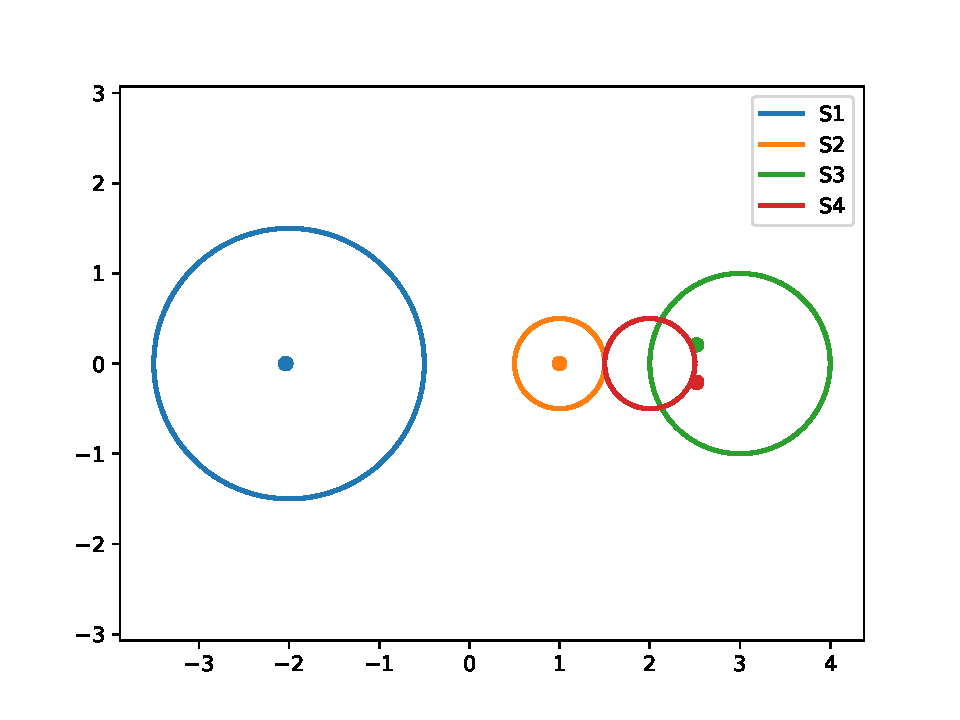
\includegraphics[scale = .4]{Oppgave_3A_plot.pdf}
      \caption{Plot av egensirklene til matrisen $ A $ og dets egenverdier}
      \label{fig:Matrix A}
    \end{figure}



    \subsection*{b)}

    \[
        B = \begin{bmatrix*}[r]
         5 & -1 & 1 \\
         1 & 2 & 1 \\
         1 & -1 & -1 \\
        \end{bmatrix*}
    \]

      \begin{figure}[h!]
        \centering
        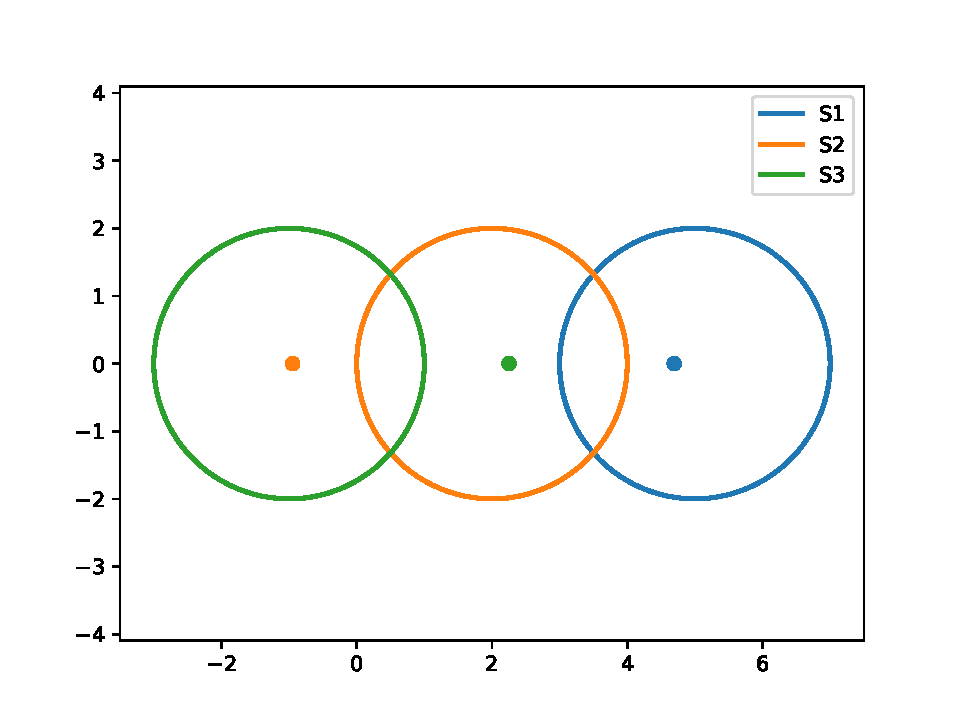
\includegraphics[scale = .4]{Oppgave_3B_plot.pdf}
        \caption{Plot av egensirklene til matrisen $ B $ og dets egenverdier}
        \label{fig:Matrix B}
      \end{figure}

    \subsection*{c)}

      \[
      C = 
      \begin{bmatrix*}[r]
       0 & 3 & 7 & 1 & 6 \\
       7 & 10 & 1 & 7 & 9 \\
       1 & 8 & 20 & 1 & 1 \\
       1 & 9 & 3 & 30 & 3 \\
       1 & 7 & 3 & 2 & 40 \\
      \end{bmatrix*}
      \]

      \begin{figure}[h!]
        \centering
        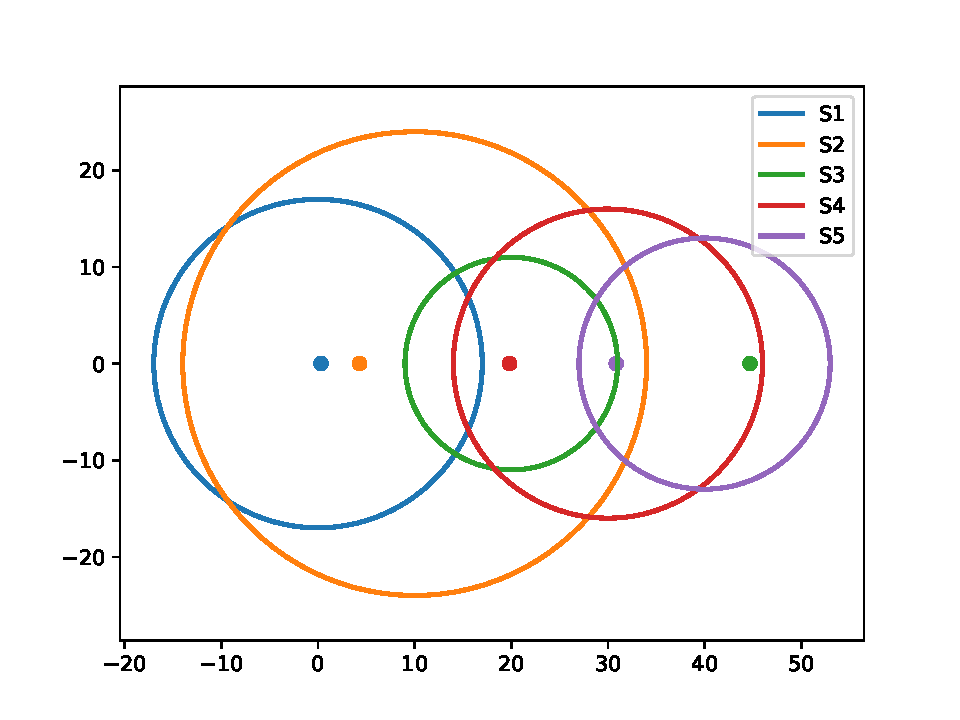
\includegraphics[scale = .4]{Oppgave_3C_plot.pdf}
        \caption{Plot av egensirklene til matrisen $ C $ og dets egenverdier }
        \label{fig:Matrix C}
      \end{figure}
    
    \subsection*{d)}
      \[
      D = 
      \begin{bmatrix*}[r]
       1 & 0 & 0 & 0 \\
       0 & 6 & 0 & 0 \\
       0 & 0 & 11 & 0 \\
       0 & 0 & 0 & 16 \\
      \end{bmatrix*}
      \]
    

      \begin{figure}[h!]
        \centering
        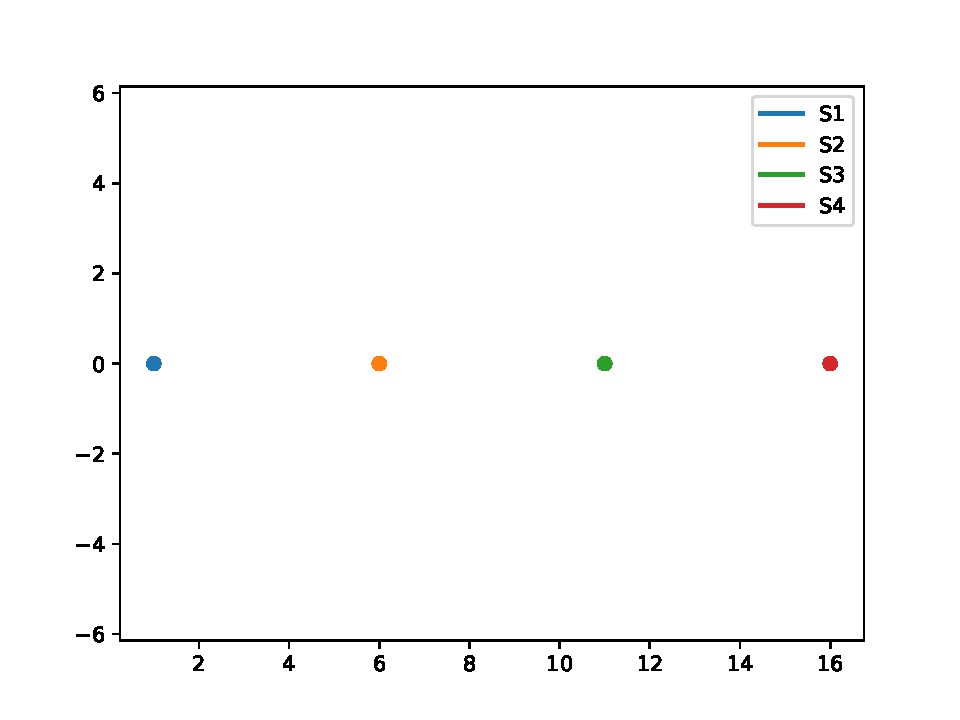
\includegraphics[scale = .4]{Oppgave_3D_plot.pdf}
        \caption{Plot av egensirklene sin matrise $ D $ og dets egenverdier}
        \label{fig:figure1}
      \end{figure}
    Egensirklene har radius $ r = 0 $ ettersom matrisen ikke har verdier utenom på diagonalen. Egenverdiene er reelle og ligger i sentrum av sirklene. 

\section*{Oppgave 4}
  \subsection*{a)}
    Egenverdiene befinner seg innenfor en av egensirklene. 
  
  \subsection*{b)}
  \[
  A \mathbf{v} = λ \mathbf{v}
  \]
  Kan skrives som 
  \[
  \sum_{j} a_{ij}v_j = λ v_i
  \]
  Hvis vi trekker ut leddet $ a_{ii} $ kan vi flytte det til den andre siden av likningen. 
  \[
  \sum_{j \neq i} a_{ij} v_{j} = (λ - a_{ii}) v_i
  \]  
  \[
  \sum_{j \neq i} \frac{a_{ij }v_j}{v_i} = \lambda - v_{ii}
  \]
  Vi bruker trekantulikheten
  \[
  \left\vert \lambda - a _{ii} \right|  = \left\vert \sum_{j \neq i} \frac{a_{ij } v_j}{v_i} \right\vert \le \sum_{j \neq i} \left\vert a_{ij } \right\vert = r_j
  \]

\section*{Oppgave 5}
  Ettersom en $ n × n $ matrise er inverterbar så lenge 0 ikke er en egenverdi, må vi vise at ingen diagonaldominant matrise har egenverdi 0 for å vise at de alltid er inverterbare. Vi beviser dette ved å sette inn $ λ = 0  $ i beviset ført i forrige oppgave. 
  \[
  \left\vert a_{ii } \right\vert \le \sum_{j \neq i} \left\vert a_{ij } \right\vert 
  \]
  Dette strider i mot definisjonen av en diagonaldominant matrise og kan dermed ikke stemme. Konklusjonen er at $ \lambda \neq 0 $. 

\section*{Oppgave 6}
  \[A=
  \begin{bmatrix*}[r]
   5 & 2 \\
   -7 & -3 \\
  \end{bmatrix*}
  \]

  \[ A^{-1} = 
    \begin{bmatrix}
      5 & 2 \\
      -7 & -3 \\
     \end{bmatrix}^{-1} = \begin{bmatrix}3 & 2\\-7 & -5\end{bmatrix}
  \]

\lstinputlisting{MAT1120 Oblig 1.py}

\end{document}